\documentclass[12pt,a4paper]{article}
\usepackage{amssymb} %mathbb
\usepackage{amsmath} %align
\usepackage{graphicx} %jpg
\usepackage[a4paper,top=1.3cm,bottom=1.3cm,left=1.3cm,right=1.3cm]{geometry}
\pagestyle{headings}
\date{}
\begin{document}
	\Large

	\begin{center}
		Terceira prova de An\'alise II

		Vin\'icius Claudino Ferraz
	\end{center}

	\normalsize

	\section{Quest\~ao 1}
		\begin{flushright}
		\end{flushright}

		Seja $R \subset \mathbb{R}^2$ a regi\~ao delimitada pelas retas $y = b$, $x = a$ e $y = x$.

		\begin{center}
		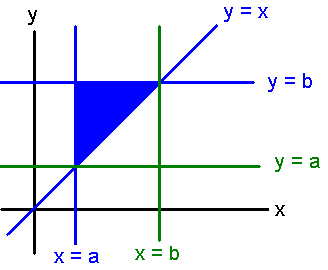
\includegraphics[scale=.5]{questao1}
		\end{center}

		\begin{align}
				I_1 &= \iint_R f = \iint_{[a, b]^2} f \cdot \chi_R = \iint_{[a, b]^2} g \\
				\chi_R(x, y) &= 1, \mathrm{\,se\,} (x, y) \in R \\
				\chi_R(x, y) &= 0, \mathrm{\,se\,} (x, y) \notin R
		\end{align}

		$f$ \'e integr\'avel $\Rightarrow$ o conjunto $D_1$ dos pontos de descontinuidade de $f$ tem medida nula.

		O conjunto $D_2$ dos pontos de descontinuidade de $\chi_R$ \'e formado pelos pontos de $\partial R$, a fronteira de $R$. $D_2$ \'e composto de tr\^es segmentos, ou seja, as arestas do tri\^angulo $\Delta ABC$, em que $A = (a, a), B = (a, b), C = (b, b)$.

		$\dim D_2 = 1 < 2 = \dim [a, b]^2 \Rightarrow D_2$ tem medida nula em $[a,b]^2$.

		Logo, o produto $f \cdot \chi_R = g$ \'e integr\'avel (uma vez que os pontos de continuidade de cada fator tem medida nula). Se $f$ \'e limitada, ent\~ao $g$ \'e limitada.

		Pelo teorema de Fubini, existem as integrais iteradas e elas se igualam a $I_1$.

		\begin{align}
				I_1 &= \int_{[a,b]} \int_{[a,b]} g = \int_{[a,b]} \biggl( \int_{[a,b]} f(x,y) \cdot \chi_R(x,y) \,\mathrm{d}x \biggl) \,\mathrm{d}y  = \int_{y = a}^{y = b} \biggl( \int_{x = a}^{x = y} f(x,y) \,\mathrm{d}x \biggl) \,\mathrm{d}y = I_2 \\
				I_1 &= \int_{[a,b]} \int_{[a,b]} g = \int_{[a,b]} \biggl( \int_{[a,b]} f(x,y) \cdot \chi_R(x,y) \,\mathrm{d}y \biggl) \,\mathrm{d}x  = \int_{x = a}^{x = b} \biggl( \int_{y = x}^{y = b} f(x,y) \,\mathrm{d}y \biggl) \,\mathrm{d}x = I_3
		\end{align}

		Portanto, $I_2 = I_3$.

		\begin{flushright}
		\end{flushright}

		\begin{flushright}
		\end{flushright}

		\begin{flushright}
		\end{flushright}

	\section{Quest\~ao 2}
		\begin{align}
			f : A \subset \mathbb{R}^n &\rightarrow \mathbb{R} \\
			x = \begin{pmatrix} x_1 \\ \vdots \\ x_n \end{pmatrix} \in \mathbb{R}^n &\Rightarrow f(x) \in \mathbb{R} \\
			\mathrm{D}f : \mathbb{R}^n &\rightarrow \mathcal{L}(\mathbb{R}^n ; \mathbb{R}) \\
			p \in \mathbb{R}^n &\Rightarrow \mathrm{D}f(p) \in \mathcal{L}(\mathbb{R}^n ; \mathbb{R}) \\
			\mathrm{D}f(p) : \mathbb{R}^n &\rightarrow \mathbb{R} \\
			v = \begin{pmatrix} v_1 \\ \vdots \\ v_n \end{pmatrix} \in \mathbb{R}^n &\Rightarrow \mathrm{D}f(p)(v) \in \mathbb{R} \\
			\mathrm{D}f(p)(v) &= \frac{\partial f}{\partial x_1} (p) v_1 + ... + \frac{\partial f}{\partial x_n} (p) v_n \\
			x_i : \mathbb{R}^n &\rightarrow \mathbb{R} ; \begin{pmatrix} x_1 \\ \vdots \\ x_n \end{pmatrix} \mapsto x_i \\
			\mathrm{D}x_i : \mathbb{R}^n &\rightarrow \mathcal{L}(\mathbb{R}^n ; \mathbb{R}) \\
			\mathrm{D}x_i (p) &= \varphi_i : \mathbb{R}^n \rightarrow \mathbb{R} \\
			\mathrm{D}x_i (p) (v) &= \varphi_i (v) = v_i \\
			\varphi_i = [\delta_{ij}]_{1 \times n} \in \mathcal{M}_{1 \times n} &\Leftrightarrow \varphi_i (v) = [0,...,1,...,0]_{1 \times n} \cdot \begin{pmatrix} v_1 \\ \vdots \\ v_n \end{pmatrix}_{n \times 1} = v_i \\
			\mathrm{d}f : A \subset \mathbb{R}^n &\rightarrow \Lambda^1(\mathbb{R}^n) = (\mathbb{R}^n)^* = \mathcal{L}(\mathbb{R}^n ; \mathbb{R}) \\
			\mathrm{d}f (p) (v) &= \mathrm{D}f(p) (v) \\
			\mathrm{d}x_i : \mathbb{R}^n &\rightarrow \Lambda^1(\mathbb{R}^n) \\
			\mathrm{d}x_i (p) (v) &= \mathrm{D}x_i(p) (v) = v_i
		\end{align}

		Pela defini\c{c}\~ao de D$f(p)(v)$:

		\begin{align}
			\mathrm{d}f(p)(v) &= \frac{\partial f}{\partial x_1} (p) v_1 + ... + \frac{\partial f}{\partial x_n} (p) v_n
		\end{align}

		Pela defini\c{c}\~ao de d$x_i(p)(v)$:

		\begin{align}
			\mathrm{d}f(p)(v) &= \frac{\partial f}{\partial x_1} (p) \mathrm{d}x_1 (p) (v) + ... + \frac{\partial f}{\partial x_n} (p) \mathrm{d}x_n (p) (v)
		\end{align}

		Como a linha acima vale $\forall v \in \mathbb{R}^n$, temos igualdade de aplica\c{c}\~oes de $\mathbb{R}^n$ em $\mathbb{R}$:

		\begin{align}
			\mathrm{d}f(p) &= \frac{\partial f}{\partial x_1} (p) \varphi_1 + ... + \frac{\partial f}{\partial x_n} (p) \varphi_n \\
			\Leftrightarrow \mathrm{d}f(p) &= \frac{\partial f}{\partial x_1} (p) \mathrm{d}x_1 (p) + ... + \frac{\partial f}{\partial x_n} (p) \mathrm{d}x_n (p)
		\end{align}

		Como a linha acima vale $\forall p \in \mathbb{R}^n$, temos igualdade de aplica\c{c}\~oes de $\mathbb{R}^n$ em $\Lambda^1(\mathbb{R}^n)$:

		\begin{align}
			\mathrm{d}f &= \frac{\partial f}{\partial x_1} \mathrm{d}x_1 + ... + \frac{\partial f}{\partial x_n} \mathrm{d}x_n
		\end{align}

	\section{Quest\~ao 3}

		\begin{align}
			\omega &= f \,\mathrm{d}x \wedge \,\mathrm{d}y \\
			c : [0,1]^2 &\rightarrow \mathbb{R}^2 ; \begin{pmatrix} u \\ v \end{pmatrix} \mapsto \begin{pmatrix} c_1(u,v) \\ c_2(u,v) \end{pmatrix}
		\end{align}

		Pela defini\c{c}\~ao de $\omega$:

		\begin{align}
			c^*\omega &= c^*(f \,\mathrm{d}x \wedge \,\mathrm{d}y)
		\end{align}

		Utilizamos a propriedade 1: $f^*(g \omega) = (g \circ f) f^*\omega$, v\'alida para toda $k$-forma $\omega$ em $\mathbb{R}^n$, para toda $f : \mathbb{R}^a \rightarrow \mathbb{R}^b$ e para toda $g : \mathbb{R}^b \rightarrow \mathbb{R}^p$.

		\begin{align}
			c^*\omega &= (f \circ c) c^*(\mathrm{d}x \wedge \,\mathrm{d}y)
		\end{align}

		Utilizamos a propriedade 2: $f^*(\omega \wedge \theta) = f^*\omega \wedge f^*\theta$, v\'alida para toda $k$-forma $\omega$ em $\mathbb{R}^n$, para toda $\ell$-forma $\theta$ em $\mathbb{R}^n$ e para toda $f : \mathbb{R}^a \rightarrow \mathbb{R}^b$.

		\begin{align}
			c^*\omega &= (f \circ c) c^*(\mathrm{d}x) \wedge c^*(\mathrm{d}y)
		\end{align}

		Utilizamos a propriedade 3: $f^*(\mathrm{d}x_i) = \sum_{j = 1}^m \frac{\partial f_i}{\partial t_j} \,\mathrm{d}t_j$, v\'alida para toda $f : \mathbb{R}^m \rightarrow \mathbb{R}^n$, para todo $(x_1, ..., x_n) \in \mathbb{R}^n$, e para todo $(t_1, ..., t_m) \in \mathbb{R}^m$.

		\begin{align}
			c^*\omega &= (f \circ c) \biggl(\frac{\partial c_1}{\partial u}\mathrm{d}u + \frac{\partial c_1}{\partial v}\mathrm{d}v\biggl) \wedge \biggl(\frac{\partial c_2}{\partial u}\mathrm{d}u + \frac{\partial c_2}{\partial v}\mathrm{d}v \biggl)
		\end{align}

		Utilizamos a propriedade distributiva do produto exterior.

		$(\omega + \theta) \wedge \varphi = \omega \wedge \varphi + \theta \wedge \varphi$, para toda $k$-forma $\omega, \theta$ em $\mathbb{R}^n$ e para toda $\ell$-forma $\varphi$ em $\mathbb{R}^n$.

		$\omega + (\theta \wedge \varphi) = \omega \wedge \theta + \omega \wedge \varphi$, para toda $k$-forma $\omega$ em $\mathbb{R}^n$ e para toda $\ell$-forma $\theta, \varphi$ em $\mathbb{R}^n$.

		\begin{align}
			c^*\omega = (f \circ c) \biggl[ &\biggl(\frac{\partial c_1}{\partial u}\mathrm{d}u\biggl) \wedge \biggl(\frac{\partial c_2}{\partial u}\mathrm{d}u \biggl)
			+ \biggl(\frac{\partial c_1}{\partial u}\mathrm{d}u\biggl) \wedge \biggl(\frac{\partial c_2}{\partial v}\mathrm{d}v \biggl) \\
			+ &\biggl(\frac{\partial c_1}{\partial v}\mathrm{d}v\biggl) \wedge \biggl(\frac{\partial c_2}{\partial u}\mathrm{d}u \biggl)
			+ \biggl(\frac{\partial c_1}{\partial v}\mathrm{d}v\biggl) \wedge \biggl(\frac{\partial c_2}{\partial v}\mathrm{d}v \biggl) \biggl]
		\end{align}

		Utilizamos a multiplica\c{c}\~ao por escalar: $(a\omega) \wedge \theta = \omega \wedge (a \theta) = a (\omega \wedge \theta)$, v\'alida para toda $k$-forma $\omega$ em $\mathbb{R}^n$, para toda $\ell$-forma $\theta$ em $\mathbb{R}^n$ e para todo $a \in \mathbb{R}$.

		\begin{align}
			c^*\omega = (f \circ c) \biggl[ &\frac{\partial c_1}{\partial u} \frac{\partial c_2}{\partial u}\,\mathrm{d}u \wedge \mathrm{d}u
			+ \frac{\partial c_1}{\partial u} \frac{\partial c_2}{\partial v}\,\mathrm{d}u \wedge \mathrm{d}v
			+ \frac{\partial c_1}{\partial v} \frac{\partial c_2}{\partial u}\,\mathrm{d}v \wedge \mathrm{d}u
			+ \frac{\partial c_1}{\partial v} \frac{\partial c_2}{\partial v}\,\mathrm{d}v \wedge \mathrm{d}v \biggl]
		\end{align}

		Utilizamos a identidade $\omega \wedge \omega = 0$, v\'alida para 1-formas $\omega$ em $\mathbb{R}^n$.

		\begin{align}
			c^*\omega = (f \circ c) \biggl[ &\frac{\partial c_1}{\partial u} \frac{\partial c_2}{\partial v}\,\mathrm{d}u \wedge \mathrm{d}v
			+ \frac{\partial c_1}{\partial v} \frac{\partial c_2}{\partial u}\,\mathrm{d}v \wedge \mathrm{d}u \biggl]
		\end{align}

		Utilizamos a identidade $\omega \wedge \theta = (-1)^{k\ell} \theta \wedge \omega$, v\'alida para toda $k$-forma $\omega$ em $\mathbb{R}^n$ e para toda $\ell$-forma $\theta$ em $\mathbb{R}^n$.

		\begin{align}
			c^*\omega = (f \circ c) \biggl[ &\frac{\partial c_1}{\partial u} \frac{\partial c_2}{\partial v}
			- \frac{\partial c_1}{\partial v} \frac{\partial c_2}{\partial u} \biggl] \,\mathrm{d}u \wedge \mathrm{d}v
		\end{align}

	\section{Quest\~ao 4}
		\begin{flushright}
		\end{flushright}

		Escrever a demonstra\c{c}\~ao do teorema de Stokes para uma 2-forma e um 3-cubo de $\mathbb{R}^3$ e comparar com o teorema da diverg\^encia.

		\begin{flushright}
		\end{flushright}

		Sejam as fun\c{c}\~oes $F, G, H : \mathbb{R}^3 \rightarrow \mathbb{R}$ de classe $C^\infty$.

		Seja $p = \begin{pmatrix} x_1 \\ x_2 \\ x_3 \end{pmatrix} \in \mathbb{R}^3$.

		Seja $\omega$ uma 2-forma em $\mathbb{R}^3$:

		\begin{align}
			\omega(p) &= F(p) \,\mathrm{d}x_1 \wedge \mathrm{d}x_2 + G(p) \,\mathrm{d}x_1 \wedge \mathrm{d}x_3 + H(p) \,\mathrm{d}x_2 \wedge \mathrm{d}x_3 \label{DefinaOmega} \\
			\omega_1 &= F \,\mathrm{d}x_1 \wedge\mathrm{d}x_2 \Rightarrow \mathrm{d}\omega_1 = \frac{\partial F}{\partial x_3} \,\mathrm{d}x_3 \wedge\mathrm{d}x_1 \wedge\mathrm{d}x_2 \\
			\omega_2 &= G \,\mathrm{d}x_1 \wedge\mathrm{d}x_3 \Rightarrow \mathrm{d}\omega_2 = \frac{\partial G}{\partial x_2} \,\mathrm{d}x_2 \wedge\mathrm{d}x_1 \wedge\mathrm{d}x_3 \\
			\omega_3 &= H \,\mathrm{d}x_2 \wedge\mathrm{d}x_3 \Rightarrow \mathrm{d}\omega_3 = \frac{\partial H}{\partial x_1} \,\mathrm{d}x_1 \wedge\mathrm{d}x_2 \wedge\mathrm{d}x_3 \\
			\mathrm {Logo,\,\,} \omega &= \omega_1 + \omega_2 + \omega_3 \label{DecomposicaoOmega} \\
			\mathrm{d}\omega &= \biggl( \frac{\partial F}{\partial x_3} - \frac{\partial G}{\partial x_2} + \frac{\partial H}{\partial x_1} \biggl) \,\mathrm{d}x_1 \wedge\mathrm{d}x_2 \wedge\mathrm{d}x_3
		\end{align}

		Sejam $t_1, t_2, t_3 \in \mathbb{R}$. E seja $c$ um 3-cubo de $\mathbb{R}^3$ tal que

		\begin{align}
			c : [0,1]^3 \rightarrow \mathbb{R}^3 ;  \begin{pmatrix} t_1 \\ t_2 \\ t_3 \end{pmatrix} \mapsto \begin{bmatrix} c_1(t_1, t_2, t_3) \\ c_2(t_1, t_2, t_3) \\ c_3(t_1, t_2, t_3) \end{bmatrix}
		\end{align}

	\subsection{Enunciado do Teorema de Stokes}
		\begin{flushright}
		\end{flushright}

		Seja $\omega$ uma $(k-1)$-forma em $\mathbb{R}^n$ e seja $c$ um $k$-cubo em $\mathbb{R}^n$. Ent\~ao:

		\begin{align}
			\int_c \,\mathrm{d}\omega = \int_{\partial c} \omega
		\end{align}

		Em particular, fixado $\omega$ como na linha (\ref{DefinaOmega}),

		\begin{align}
			\int_c \biggl( \frac{\partial F}{\partial x_3} - \frac{\partial G}{\partial x_2} + \frac{\partial H}{\partial x_1} \biggl) \,\mathrm{d}x_1 \wedge\mathrm{d}x_2 \wedge\mathrm{d}x_3 = \int_{\partial c} F \,\mathrm{d}x_1 \wedge \mathrm{d}x_2 + G \,\mathrm{d}x_1 \wedge \mathrm{d}x_3 + H \,\mathrm{d}x_2 \wedge \mathrm{d}x_3 \label{Quatorze}
		\end{align}

		Em geral, o teorema de Stokes vale para uma $k$-cadeia $C$.

		Sejam os $k$-cubos $c_i, i \in \{ 1, 2, ..., \ell \}, \ell \in \mathbb{N}, z_i \in \mathbb{Z}$.

		\begin{align}
			C &= \sum_{i = 1}^\ell z_i c_i \\
			\int_C \,\mathrm{d}\omega &= \int_{\partial C} \omega
		\end{align}

	\subsection{Enunciado do Teorema da Diverg\^encia}
		\begin{flushright}
		\end{flushright}

		Seja $\Phi$ uma aplica\c{c}\~ao de classe $C^\infty$ tal que $\Phi : \mathbb{R}^3 \rightarrow \mathbb{R}^3 ; (p) \mapsto \begin{bmatrix} \Phi_1(p) \\ \Phi_2(p) \\ \Phi_3(p) \end{bmatrix}$.

		Seja $n$ vetor normal a $c$, orientado de forma a apontar sempre para fora. Ent\~ao:

		\begin{align}
			\int_c \langle \nabla , \Phi \rangle \,\mathrm{d}V &= \int_{\partial c} \langle \Phi , n \rangle \,\mathrm{d}A \\
			\langle \nabla , \Phi \rangle &= \langle (\mathrm{D}x_1, \mathrm{D}x_2, \mathrm{D}x_3), (\Phi_1, \Phi_2, \Phi_3) \rangle \\
			\langle \Phi , n \rangle \,\mathrm{d}A &= \Phi_1 (n_1 \,\mathrm{d}A) + \Phi_2 (n_2 \,\mathrm{d}A) + \Phi_3 (n_3 \,\mathrm{d}A) \\
			\mathrm{Ou\,seja,\,} \int_c \,\mathrm{d}\theta &= \int_{\partial c} \theta \\
			\theta &= \Phi_1 \,\mathrm{d}x_2 \wedge\mathrm{d}x_3 + \Phi_2 \,\mathrm{d}x_3 \wedge\mathrm{d}x_1 + \Phi_3 \,\mathrm{d}x_1 \wedge\mathrm{d}x_2
		\end{align}

		Para passar do enunciado do exerc\'icio para o teorema da diverg\^encia, basta fazermos

		\begin{align}
			\Phi_1 = H, \Phi_2 = -G, \Phi_3 = F
		\end{align}

		em (\ref{Quatorze}) e assim obteremos

		\begin{align}
			\int_c \biggl( \frac{\partial \Phi_3}{\partial x_3} + \frac{\partial \Phi_2}{\partial x_2} + \frac{\partial \Phi_1}{\partial x_1} \biggl) \,\mathrm{d}x_1 \wedge\mathrm{d}x_2 \wedge\mathrm{d}x_3 = \int_{\partial c} \Phi_3 \,\mathrm{d}x_1 \wedge \mathrm{d}x_2 - \Phi_2 \,\mathrm{d}x_1 \wedge \mathrm{d}x_3 + \Phi_1 \,\mathrm{d}x_2 \wedge \mathrm{d}x_3
		\end{align}

		\begin{flushright}
		\end{flushright}

		Redigiremos agora a demonstra\c{c}\~ao requisitada.

		\begin{align}
			\int_c \,\mathrm{d}\omega &\stackrel{\ref{VinteDois}.1}{=} \int_{[0, 1]^3} c^*(\mathrm{d}\omega) \stackrel{\ref{VinteDois}.2}{=} \underbrace{\int_{I^3} \,\mathrm{d}(c^*\omega)}_\text{$T$} \stackrel{\ref{VinteDois}.3}{=} \underbrace{\int_{\partial I^3} c^*\omega}_\text{$S$} \stackrel{\ref{VinteDois}.4}{=} \sum_{i,\alpha} (-1)^{i + \alpha} \int_{I_{(i, \alpha)}^3} c^*\omega \stackrel{\ref{VinteDois}.5}{=} \label{VinteDois} \\
				&\stackrel{\ref{VinteDois}.5}{=} \sum_{i,\alpha} (-1)^{i + \alpha} \int_{[0,1]^2} c_{(i, \alpha)}^* \omega \stackrel{\ref{VinteDois}.6}{=} \sum_{i,\alpha} (-1)^{i + \alpha} \int_{c(i,\alpha)} \omega \stackrel{\ref{VinteDois}.7}{=} \int_{\partial c} \omega
		\end{align}

		Consideremos inicialmente a parcela $\omega_1$ na decomposi\c{c}\~ao em (\ref{DecomposicaoOmega}).

		\ref{VinteDois}.1 segue da defini\c{c}\~ao de integral:

		\begin{align}
			c^*(\mathrm{d}\omega_1) &= c^*\biggl(\frac{\partial F}{\partial x_3} \,\mathrm{d}x_1 \wedge\mathrm{d}x_2 \wedge\mathrm{d}x_3\biggl) = \biggl( \frac{\partial F}{\partial x_3} \circ c \biggl) c^*(\mathrm{d}x_1) \wedge c^*(\mathrm{d}x_2) \wedge c^* (\mathrm{d}x_3) \\
			c^*(\mathrm{d}\omega_1) &= \biggl( \frac{\partial F}{\partial x_3} \circ c \biggl) \biggl(\frac{\partial c_1}{\partial t_1} \,\mathrm{d}t_1 + \frac{\partial c_1}{\partial t_2} \,\mathrm{d}t_2 + \frac{\partial c_1}{\partial t_3} \,\mathrm{d}t_3 \biggl)
				\wedge \biggl(\frac{\partial c_2}{\partial t_1} \,\mathrm{d}t_1 + \frac{\partial c_2}{\partial t_2} \,\mathrm{d}t_2 + \frac{\partial c_2}{\partial t_3} \,\mathrm{d}t_3 \biggl) \wedge \\
				&\wedge \biggl(\frac{\partial c_3}{\partial t_1} \,\mathrm{d}t_1 + \frac{\partial c_3}{\partial t_2} \,\mathrm{d}t_2 + \frac{\partial c_3}{\partial t_3} \,\mathrm{d}t_3 \biggl)  \\
			c^*(\mathrm{d}\omega_1) &= \biggl( \frac{\partial F}{\partial x_3} \circ c \biggl) \biggl(\frac{\partial c_1}{\partial t_1} \frac{\partial c_2}{\partial t_2} \frac{\partial c_3}{\partial t_3}
				- \frac{\partial c_1}{\partial t_1} \frac{\partial c_3}{\partial t_2} \frac{\partial c_2}{\partial t_3}
				- \frac{\partial c_2}{\partial t_1} \frac{\partial c_1}{\partial t_2} \frac{\partial c_3}{\partial t_3}
				+ \frac{\partial c_2}{\partial t_1} \frac{\partial c_3}{\partial t_2} \frac{\partial c_1}{\partial t_3} \\
				&+ \frac{\partial c_3}{\partial t_1} \frac{\partial c_1}{\partial t_2} \frac{\partial c_2}{\partial t_3}
				- \frac{\partial c_3}{\partial t_1} \frac{\partial c_2}{\partial t_2} \frac{\partial c_1}{\partial t_3}	\biggl) \,\mathrm{d}t_1 \wedge \mathrm{d}t_2 \wedge \mathrm{d}t_3
		\end{align}

		\ref{VinteDois}.2 segue da seguinte propriedade: pull-back de diferencial \'e igual a diferencial de pull-back.

		\begin{align}
			c^*\omega_1 &= c^*(F \,\mathrm{d}x_1 \wedge\mathrm{d}x_2) = (F \circ c) c^*(\mathrm{d}x_1) \wedge c^*(\mathrm{d}x_2) \label{VinteNove} \\
			c^*\omega_1 &= (F \circ c) \biggl(\frac{\partial c_1}{\partial t_1} \,\mathrm{d}t_1 + \frac{\partial c_1}{\partial t_2} \,\mathrm{d}t_2 + \frac{\partial c_1}{\partial t_3} \,\mathrm{d}t_3 \biggl)
				\wedge \biggl(\frac{\partial c_2}{\partial t_1} \,\mathrm{d}t_1 + \frac{\partial c_2}{\partial t_2} \,\mathrm{d}t_2 + \frac{\partial c_2}{\partial t_3} \,\mathrm{d}t_3 \biggl) \\
			c^*\omega_1 &= (F \circ c) \biggl(\frac{\partial c_1}{\partial t_1} \frac{\partial c_2}{\partial t_2} - \frac{\partial c_2}{\partial t_1} \frac{\partial c_1}{\partial t_2} \biggl) \,\mathrm{d}t_1 \wedge \mathrm{d}t_2
				+ (F \circ c) \biggl(\frac{\partial c_1}{\partial t_1} \frac{\partial c_2}{\partial t_3} - \frac{\partial c_2}{\partial t_1} \frac{\partial c_1}{\partial t_3} \biggl) \,\mathrm{d}t_1 \wedge \mathrm{d}t_3 \\
				&+ (F \circ c) \biggl(\frac{\partial c_1}{\partial t_2} \frac{\partial c_2}{\partial t_3} - \frac{\partial c_2}{\partial t_2} \frac{\partial c_1}{\partial t_3} \biggl) \,\mathrm{d}t_2 \wedge \mathrm{d}t_3
		\end{align}

		Seja agora mais uma decomposi\c{c}\~ao:

		\begin{align}
			f &= (F \circ c) \biggl(\frac{\partial c_1}{\partial t_1} \frac{\partial c_2}{\partial t_2} - \frac{\partial c_2}{\partial t_1} \frac{\partial c_1}{\partial t_2} \biggl) \\
			g &= (F \circ c) \biggl(\frac{\partial c_1}{\partial t_1} \frac{\partial c_2}{\partial t_3} - \frac{\partial c_2}{\partial t_1} \frac{\partial c_1}{\partial t_3} \biggl) \\
			h	&= (F \circ c) \biggl(\frac{\partial c_1}{\partial t_2} \frac{\partial c_2}{\partial t_3} - \frac{\partial c_2}{\partial t_2} \frac{\partial c_1}{\partial t_3} \biggl) \\
			\mathrm{Logo,\,\,} c^*\omega_1 &= f \,\mathrm{d}t_1 \wedge \mathrm{d}t_2 + g \,\mathrm{d}t_1 \wedge \mathrm{d}t_3 + h \,\mathrm{d}t_2 \wedge \mathrm{d}t_3 \\
			\mathrm{d}(c^*\omega_1) &= \biggl( \frac{\partial f}{\partial t_3} - \frac{\partial g}{\partial t_2} + \frac{\partial h}{\partial t_1} \biggl) \,\mathrm{d}t_1 \wedge \mathrm{d}t_2 \wedge \mathrm{d}t_3 \label{TrintaQuatro}
		\end{align}

		Na linha acima est\'a exibido o integrando em \ref{VinteDois}.2 ($T$). A regi\~ao de integra\c{c}\~ao \'e o cubo Identidade, definido por $I^3 = I$, por simplicidade. Seja $I : [0,1]^3 \rightarrow \mathbb{R}^3 ; p \mapsto p = I(p) = I^3(p)$.

		\begin{flushright}
		\end{flushright}

		Vamos agora provar \ref{VinteDois}.3, ou seja, $S = T$. Por linearidade, temos que

		\begin{align}
			S &= S_1 + S_2 + S_3 \\
			S_1 &= \int_{\partial I^3} f \,\mathrm{d}t_1 \wedge \mathrm{d}t_2 \\
			S_2 &= \int_{\partial I^3} g \,\mathrm{d}t_1 \wedge \mathrm{d}t_3 \\
			S_3 &= \int_{\partial I^3} h \,\mathrm{d}t_2 \wedge \mathrm{d}t_3
		\end{align}

		\begin{align}
			S_1 &= \int_{\partial I^3} f \,\mathrm{d}t_1 \wedge \mathrm{d}t_2 \stackrel{\ref{QuarentaQuatro}.1}{=} \sum_{j, \alpha} (-1)^{j + \alpha} \int_{I^3_{(j, \alpha)}} f \,\mathrm{d}t_1 \wedge \mathrm{d}t_2 \stackrel{\ref{QuarentaQuatro}.2}{=} \sum_{j, \alpha} (-1)^{j + \alpha} \int_{[0,1]^2} (I_{(j, \alpha)}^{3})^* (f \,\mathrm{d}t_1 \wedge \mathrm{d}t_2) \label{QuarentaQuatro} \\
			&\stackrel{\ref{QuarentaQuatro}.3}{=} \sum_{j, \alpha} (-1)^{j + \alpha} \int_{[0,1]^2} (f \circ I_{(j, \alpha)}) I^*_{(j, \alpha)} (\mathrm{d}t_1) \wedge I^*_{(j, \alpha)} (\mathrm{d}t_2)
		\end{align}

		\ref{QuarentaQuatro}.1 segue da defini\c{c}\~ao de bordo de I. \ref{QuarentaQuatro}.2 segue da defini\c{c}\~ao de integral.	\ref{QuarentaQuatro}.3 segue da defini\c{c}\~ao de pull-back.

		Seja $(e_1, e_2, e_3)$ a base can\^onica de $\mathbb{R}^3$. Sabemos que $I^*_{(j, \alpha)} (\mathrm{d}t_\ell) = 0$, se $\ell \neq j$, uma vez que d$t_\ell(p)(e_j) = \delta_{j\ell}$.

		Sabemos tamb\'em que $S_1$ \'e integral sem o termo d$t_3$, que est\'a faltando para completar 3-forma em $\mathbb{R}^3$. E assim s\'o aparecem os cubos bidimensionais $c(3, \alpha)$, que s\~ao faces do cubo $c$ definido no in\'icio.

		\begin{align}
			S_1 &= \sum_{\alpha = 0}^1 (-1)^{3 + \alpha} \int_{[0,1]^2} (f \circ I^3_{(3, \alpha)}) \,\mathrm{d}t_1 \wedge \mathrm{d}t_2 \\
			&= \sum_{\alpha = 0}^1 (-1)^{3 + \alpha} \int_{[0,1]^2} f(t_1, t_2, \alpha) \,\mathrm{d}t_1 \wedge \mathrm{d}t_2 \\
			&= (-1)^{3 + 1} \int_{[0,1]^2} (f(t_1, t_2, 1) - f(t_1, t_2, 0)) \,\mathrm{d}t_1 \wedge \mathrm{d}t_2 \\
			&= + \int_{[0,1]^2} \biggl[ \int_{[0,1]} \frac{\partial f}{\partial t_3} (t_1, t_2) \,\mathrm{d}t_3 \biggl] \,\mathrm{d}t_1 \wedge \mathrm{d}t_2 \\
			&= + \int_{[0,1]^3} \frac{\partial f}{\partial t_3} \,\mathrm{d}t_1 \wedge \mathrm{d}t_2 \wedge \mathrm{d}t_3 = T_1
		\end{align}

		A linha acima fez coincidir exatamente com uma parcela de (\ref{TrintaQuatro}). Por sua vez, $T_1$ no \'ultimo membro \'e parte de $T$ em (\ref{VinteDois}), restringindo-nos ainda a $\omega_1$.

		Para provar que $S = T$, basta repetir o racioc\'inio e lembrar que $T = T_1 + T_2 + T_3$.

		\begin{align}
			S_2 &= \int_{\partial I^3} g \,\mathrm{d}t_1 \wedge \mathrm{d}t_3 = \sum_{j, \alpha} (-1)^{j + \alpha} \int_{I^3_{(j, \alpha)}} g \,\mathrm{d}t_1 \wedge \mathrm{d}t_3 = \sum_{j, \alpha} (-1)^{j + \alpha} \int_{[0,1]^2} (I_{(j, \alpha)}^{3})^* (g \,\mathrm{d}t_1 \wedge \mathrm{d}t_3) \\
			&= \sum_{j, \alpha} (-1)^{j + \alpha} \int_{[0,1]^2} (g \circ I_{(j, \alpha)}) I^*_{(j, \alpha)} (\mathrm{d}t_1) \wedge I^*_{(j, \alpha)} (\mathrm{d}t_3)
		\end{align}

		Sabemos que $S_2$ \'e integral sem o termo d$t_2$, que est\'a faltando para completar 3-forma em $\mathbb{R}^3$. E assim s\'o aparecem os cubos bidimensionais $c(2, \alpha)$, que s\~ao faces do cubo $c$ definido no in\'icio.

		\begin{align}
			S_2 &= \sum_{\alpha = 0}^1 (-1)^{2 + \alpha} \int_{[0,1]^2} (g \circ I^3_{(2, \alpha)}) \,\mathrm{d}t_1 \wedge \mathrm{d}t_3 \\
			&= \sum_{\alpha = 0}^1 (-1)^{2 + \alpha} \int_{[0,1]^2} g(t_1, \alpha, t_3) \,\mathrm{d}t_1 \wedge \mathrm{d}t_3 \\
			&= (-1)^{2 + 1} \int_{[0,1]^2} (g(t_1, 1, t_3) - g(t_1, 0, t_3)) \,\mathrm{d}t_1 \wedge \mathrm{d}t_3 \\
			&= - \int_{[0,1]^2} \biggl[ \int_{[0,1]} \frac{\partial g}{\partial t_2} (t_1, t_3) \,\mathrm{d}t_2 \biggl] \,\mathrm{d}t_1 \wedge \mathrm{d}t_3 \\
			&= - \int_{[0,1]^3} \frac{\partial g}{\partial t_2} \,\mathrm{d}t_1 \wedge \mathrm{d}t_2 \wedge \mathrm{d}t_3 = T_2
		\end{align}

		\begin{align}
			S_3 &= \int_{\partial I^3} h \,\mathrm{d}t_2 \wedge \mathrm{d}t_3 = \sum_{j, \alpha} (-1)^{j + \alpha} \int_{I^3_{(j, \alpha)}} h \,\mathrm{d}t_2 \wedge \mathrm{d}t_3 = \sum_{j, \alpha} (-1)^{j + \alpha} \int_{[0,1]^2} (I_{(j, \alpha)}^{3})^* (h \,\mathrm{d}t_2 \wedge \mathrm{d}t_3) \\
			&= \sum_{j, \alpha} (-1)^{j + \alpha} \int_{[0,1]^2} (h \circ I_{(j, \alpha)}) I^*_{(j, \alpha)} (\mathrm{d}t_2) \wedge I^*_{(j, \alpha)} (\mathrm{d}t_3)
		\end{align}

		Sabemos que $S_3$ \'e integral sem o termo d$t_1$, que est\'a faltando para completar 3-forma em $\mathbb{R}^3$. E assim s\'o aparecem os cubos bidimensionais $c(1, \alpha)$, que s\~ao faces do cubo $c$ definido no in\'icio.

		\begin{align}
			S_3 &= \sum_{\alpha = 0}^1 (-1)^{1 + \alpha} \int_{[0,1]^2} (h \circ I^3_{(1, \alpha)}) \,\mathrm{d}t_2 \wedge \mathrm{d}t_3 \\
			&= \sum_{\alpha = 0}^1 (-1)^{1 + \alpha} \int_{[0,1]^2} h(\alpha, t_2, t_3) \,\mathrm{d}t_2 \wedge \mathrm{d}t_3 \\
			&= (-1)^{1 + 1} \int_{[0,1]^2} (h(1, t_2, t_3) - h(0, t_2, t_3)) \,\mathrm{d}t_2 \wedge \mathrm{d}t_3 \\
			&= + \int_{[0,1]^2} \biggl[ \int_{[0,1]} \frac{\partial h}{\partial t_1} (t_2, t_3) \,\mathrm{d}t_1 \biggl] \,\mathrm{d}t_2 \wedge \mathrm{d}t_3 \\
			&= + \int_{[0,1]^3} \frac{\partial h}{\partial t_1} \,\mathrm{d}t_1 \wedge \mathrm{d}t_2 \wedge \mathrm{d}t_3 = T_3
		\end{align}

		Logo, $S(\omega_1) = T(\omega_1)$.

		Para completar nosso trabalho, resta considerar $\omega_2$ e $\omega_3$ a partir de (\ref{VinteNove}).

		\begin{align}
			c^*\omega_2 &= c^*(G \,\mathrm{d}x_1 \wedge\mathrm{d}x_3) = (G \circ c) c^*(\mathrm{d}x_1) \wedge c^*(\mathrm{d}x_3) \\
			c^*\omega_2 &= (G \circ c) \biggl(\frac{\partial c_1}{\partial t_1} \,\mathrm{d}t_1 + \frac{\partial c_1}{\partial t_2} \,\mathrm{d}t_2 + \frac{\partial c_1}{\partial t_3} \,\mathrm{d}t_3 \biggl)
				\wedge \biggl(\frac{\partial c_3}{\partial t_1} \,\mathrm{d}t_1 + \frac{\partial c_3}{\partial t_2} \,\mathrm{d}t_2 + \frac{\partial c_3}{\partial t_3} \,\mathrm{d}t_3 \biggl) \\
			c^*\omega_2 &= \underbrace{(G \circ c) \biggl(\frac{\partial c_1}{\partial t_1} \frac{\partial c_3}{\partial t_2} - \frac{\partial c_3}{\partial t_1} \frac{\partial c_1}{\partial t_2} \biggl)}_\text{$f_2$} \,\mathrm{d}t_1 \wedge \mathrm{d}t_2
				+ \underbrace{(G \circ c) \biggl(\frac{\partial c_1}{\partial t_1} \frac{\partial c_3}{\partial t_3} - \frac{\partial c_3}{\partial t_1} \frac{\partial c_1}{\partial t_3} \biggl)}_\text{$g_2$} \,\mathrm{d}t_1 \wedge \mathrm{d}t_3 \\
				&+ \underbrace{(G \circ c) \biggl(\frac{\partial c_1}{\partial t_2} \frac{\partial c_3}{\partial t_3} - \frac{\partial c_3}{\partial t_2} \frac{\partial c_1}{\partial t_3} \biggl)}_\text{$h_2$} \,\mathrm{d}t_2 \wedge \mathrm{d}t_3 \\
			c^*\omega_2 &= f_2 \,\mathrm{d}t_1 \wedge \mathrm{d}t_2 + g_2 \,\mathrm{d}t_1 \wedge \mathrm{d}t_3 + h_2 \,\mathrm{d}t_2 \wedge \mathrm{d}t_3
		\end{align}

		Analogamente, $S(\omega_2) = T(\omega_2)$.

		\begin{align}
			c^*\omega_3 &= c^*(H \,\mathrm{d}x_2 \wedge\mathrm{d}x_3) = (H \circ c) c^*(\mathrm{d}x_2) \wedge c^*(\mathrm{d}x_3) \\
			c^*\omega_3 &= (H \circ c) \biggl(\frac{\partial c_2}{\partial t_1} \,\mathrm{d}t_1 + \frac{\partial c_2}{\partial t_2} \,\mathrm{d}t_2 + \frac{\partial c_2}{\partial t_3} \,\mathrm{d}t_3 \biggl)
				\wedge \biggl(\frac{\partial c_3}{\partial t_1} \,\mathrm{d}t_1 + \frac{\partial c_3}{\partial t_2} \,\mathrm{d}t_2 + \frac{\partial c_3}{\partial t_3} \,\mathrm{d}t_3 \biggl) \\
			c^*\omega_3 &= (H \circ c) \biggl(\frac{\partial c_2}{\partial t_1} \frac{\partial c_3}{\partial t_2} - \frac{\partial c_3}{\partial t_1} \frac{\partial c_2}{\partial t_2} \biggl) \,\mathrm{d}t_1 \wedge \mathrm{d}t_2
				+ (H \circ c) \biggl(\frac{\partial c_2}{\partial t_1} \frac{\partial c_3}{\partial t_3} - \frac{\partial c_3}{\partial t_1} \frac{\partial c_2}{\partial t_3} \biggl) \,\mathrm{d}t_1 \wedge \mathrm{d}t_3 \\
				&+ (H \circ c) \biggl(\frac{\partial c_2}{\partial t_2} \frac{\partial c_3}{\partial t_3} - \frac{\partial c_3}{\partial t_2} \frac{\partial c_2}{\partial t_3} \biggl) \,\mathrm{d}t_2 \wedge \mathrm{d}t_3 \\
			c^*\omega_3 &= f_3 \,\mathrm{d}t_1 \wedge \mathrm{d}t_2 + g_3 \,\mathrm{d}t_1 \wedge \mathrm{d}t_3 + h_3 \,\mathrm{d}t_2 \wedge \mathrm{d}t_3
		\end{align}

		Analogamente, $S(\omega_3) = T(\omega_3)$.

		Portanto, por linearidade,

		\begin{align}
			\int_{I^3} \,\mathrm{d}(c^*(\omega_1 + \omega_2 + \omega_3)) &= \int_{\partial I^3} c^*(\omega_1 + \omega_2 + \omega_3) \\
			T(\omega_1) + T(\omega_2) + T(\omega_3) &= S(\omega_1) + S(\omega_2) + S(\omega_3) \\
			T &= S
		\end{align}

		Est\'a provado \ref{VinteDois}.3.

		\ref{VinteDois}.4 segue da defini\c{c}\~ao de bordo de $I^3$.

		\ref{VinteDois}.5 segue da defini\c{c}\~ao de integral de $c^*\omega$.

		\ref{VinteDois}.6 segue da defini\c{c}\~ao de integral de $\omega$.

		\ref{VinteDois}.7 segue da defini\c{c}\~ao de bordo de $c$.

		Conclus\~ao: por linearidade, passamos de $3$-cubos a $3$-cadeias e vale o Teorema de Stokes para $k = 3$.

\end{document}
